 \documentclass[11pt, oneside]{article}   	% use "amsart" instead of "article" for AMSLaTeX format
\usepackage{geometry}                		% See geometry.pdf to learn the layout options. There are lots.
\geometry{letterpaper}                   		% ... or a4paper or a5paper or ... 
%\geometry{landscape}                		% Activate for for rotated page geometry
%\usepackage[parfill]{parskip}    		% Activate to begin paragraphs with an empty line rather than an indent
\usepackage{graphicx}				% Use pdf, png, jpg, or eps§ with pdflatex; use eps in DVI mode
								% TeX will automatically convert eps --> pdf in pdflatex		
\usepackage{amssymb}
\usepackage{amsmath}
\usepackage{parskip}
\usepackage{color}
\usepackage{hyperref}

\title{Complex functions:  Exponential}
%\author{The Author}
%\section{}
%\subsection*{}
\date{}							% Activate to display a given date or no date

\graphicspath{{/Users/telliott_admin/Dropbox/Tex/png/}}
% \begin{center} 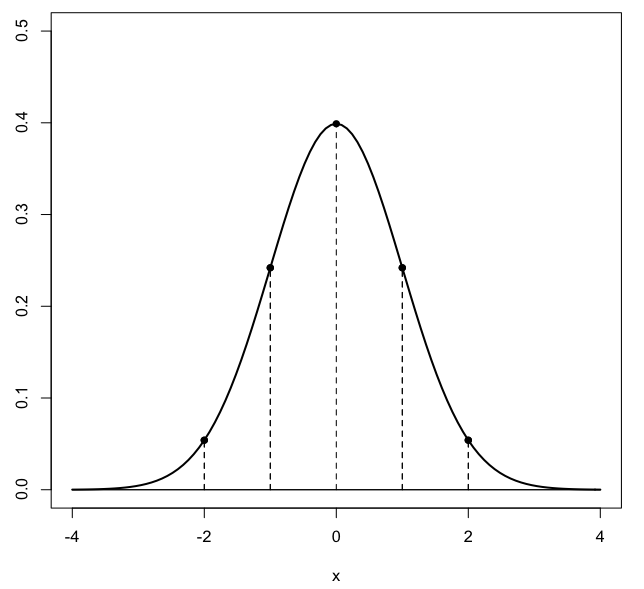
\includegraphics [scale=0.4] {gauss3.png} \end{center}
\begin{document}
\maketitle
\Large
First of all, we consider the generic complex number
\[ z = x + iy \]
and then we write
\[ f(z) = e^z \]
\[ = e^{x + iy} \]
\[ = e^x e^{iy} \]
We can thus visualize the complex exponential as having a modulus or length $e^x$ and argument or angle $\theta$ of $y$.

Then, using Euler's formula:
\[ e^x e^{iy} = e^x (\cos y + i \sin y) \]
\[ = e^x \cos y + i e^x \sin y \]

So the real part of $e^z$ is 
\[ u(x,y) = e^x \cos y \]
with partial derivatives
\[ u_x = e^x \cos y \]
\[ u_y = - e^x \sin y \]
and the imaginary part of $e^z$ is 
\[ v(x,y) = e^x \sin y \]
with partial derivatives
\[ v_x = e^x \sin y \]
\[ v_y = e^x \cos y \]
Hence
\[ u_x = e^x \cos y = v_y \]
\[ u_y = - e^x \sin y = - v_x \]
In other words, these two important conditions hold for the complex exponential:
\[ u_x = v_y \]
\[ u_y = - v_x \]
These are the famous Cauchy-Riemann equations or CR conditions.  

When the CRE are satisfied is then the function in question is a "good" function --- it is one we can do calculus with.  It has a derivative.

For this reason, the complex exponential $e^z$ is said to be analytic. 

(Which, according to Shankar, we could have predicted, since it depends only on $z$ and not on $z*$).

We showed in the previous section that we can evaluate the derivative along $\Delta y =0$ as:
\[ f'(z) = u_x + iv_x  \]
We obtain
\[ = e^x \cos y + i e^x \sin y = z \]
That is:  the exponential is its own derivative.

This is very good because we want our definitions for complex functions to give the standard results when $z$ has only a real part, i.e. when $y=0$.

Now, once more we recall Euler's formula (for a real variable $\theta$ or $x$):
\[ e^{i \theta} = \cos \theta + i \sin \theta \]
\[ e^{i x} = \cos x + i \sin x \]
Substitute $-x$ for $x$:
\[ e^{-i x} = \cos -x + i \sin -x \]
\[ = \cos x - i \sin x \]
By addition and subtraction we obtain:
\[ 2 \cos x = e^{i x} + e^{-i x} \]
\[ \cos x = \frac{1}{2} \ (e^{i x} + e^{-i x}) \]
and
\[ 2i \sin x = e^{i x} - e^{-i x} \]
\[ \sin x = \frac{1}{2i} \ (e^{i x} - e^{-i x}) \]

\subsection*{alternative derivations}

Another proof that the derivative of the complex exponential is as we would hope and expect:
\[ \frac{d}{dz} e^z = e^z \]
uses a Taylor series.  Shankar says to define $e^z$ in the same way as $e^x$.  For the real series:
\[ e^x = \sum_0^{\infty} \frac{x^n}{n!} \]
which we know converges, since the ratio of successive terms is
\[ R = \frac{x^{n+1}}{(n+1)!} \ \frac{n!}{x^n} = \frac{x}{n+1} \]
We ask, for what values of $x$ is the limit $\lim_{n \rightarrow \infty} R = 0$?  This is true for all $x$.

For the complex exponential:
\[ e^z = \sum_0^{\infty} \frac{z^n}{n!} \]
and again we see that 
\[ \frac{d}{dz} \ e^z = e^z \]
differentiating the series term by term.

Another approach (from McMahon) uses the limit definition:
\[ \frac{d}{dz} f(z) = \lim_{\Delta z \rightarrow 0} \frac{f(z + \Delta z) - f(z)}{\Delta z} \]
\[ \frac{d}{dz} e^z =  \lim_{\Delta z \rightarrow 0}  \frac{e^{z + \Delta z} - e^z}{\Delta z} \]
and just as in the real case, we factor out 
\[ =  e^z \lim_{\Delta z \rightarrow 0}  \frac{e^{\Delta z} - 1}{\Delta z} \]
This limit will turn out to be equal to $1$.  

Use Euler's formula to get this expression in $x$ and $y$:
\[ \frac{e^{\Delta z} - 1}{\Delta z} =  \frac{e^{\Delta x + i \Delta y} - 1}{\Delta x + i \Delta y} \]
\[ = \frac{e^{\Delta x} (\cos \Delta y + i \sin \Delta y) - 1}{\Delta x + i \Delta y} \]
\[ = \frac{(e^{\Delta x} \cos \Delta y - 1) + i  e^{\Delta x} \sin \Delta y}{\Delta x + i \Delta y} \]
The real part of the numerator is
\[ \lim_{\Delta x, \Delta y \rightarrow 0} e^{\Delta x} \cos \Delta y - 1 \]
Both the $\Delta x$ and the $\Delta y$ term tend to $1$ in the limit, so the entire expression for the real part of the numerator is equal to zero.  We are left with
\[ \lim_{\Delta x, \Delta y \rightarrow 0}  \frac{i  e^{\Delta x} \sin \Delta y}{\Delta x + i \Delta y} \]
The trick is that we set $x = 0$ \emph{first}
\[ \lim_{\Delta y \rightarrow 0}  \frac{i  e^0 \sin \Delta y}{0 + i \Delta y} = \lim_{\Delta y \rightarrow 0}  \frac{\sin \Delta y}{\Delta y} = 1 \]
where the last part is the famous limit from calculus.

\subsection*{other properties}

The complex exponential 
\[ e^z = e^x e^{iy} \]
has some properties that are not shared with the real exponential.  As we saw before, the angle $\theta + 2 \pi = \theta$ (and $2 \pi = 0$), so any number is really a family of numbers with different $\theta + 2 \pi k$ for integer $k$.

In particular, $e^z$ is periodic with a period of $2 \pi i$.  Additionally, it is possible for $e^z$ to be negative.  Consider that it is possible that
\[ e^z = -1 \]
as follows.  Let $z = 0 + i\pi$.  Then 
\[ e^x = e^0 = 1 \]
and
\[ e^{iy} = e^{i\pi} = -1 \]
So
\[ e^z = e^x e^{iy} = e^x(\cos y + i \sin y) = 1 (-1) = -1 \]
On the other hand, $e^z$ \textbf{cannot be zero}.
\[ e^z = e^x \cos y + i e^x \sin y = e^x(\cos y + i \sin y) \]
For $x \in \mathbb{R}$, $e^x > 0$ so the only way this could be zero would be if we can find a $y$ such that $\sin y$ and $\cos y$ were both zero.  Since there is no such $y$, we conclude that $e^z$ cannot be equal to zero.

\end{document}  